\section{Elosztott Adatbázisok}

 \textbf{Hatékonyság:} Szükséges üzenetváltások számával mérhető

\begin{center}
	\begin{tabular}{|l||c|c||l|}
 	 \hline
	  Protokoll & adat üzenet & kontroll üzenet & "X"Lock A érvényessége \\ \hline \hline
	  Wall írás & n & 2n & LOCK $A_i$ $\forall$i-re (n)\\ \cline{2-4}
	  Wall olvas & 1 & 1 & LOCK $A_i$ min 1 re  \\ \hline
	  Többségi írás & n & n+1 & LOCK $A_i$ $\frac{n+1}{2}$-re \\ \cline{2-4}
 	  Többségi olvas & 1 & n+1 & LOCK $A_i$ $\frac{n+1}{2}$-re \\ \hline
 	  K az N-ből írás & n & 2k & LOCK $A_i$ k-ra\\ \cline{2-4}
 	  K az N-ből olvas  & 1 & 2$\cdot$(n+1-k) & LOCK $A_i$ n+1-k\\
 	 \hline
	\end{tabular}
\end{center}

Eddig a lokális adategységekért az egyes csomópontok zármenedzserei feleltek.
	\begin{enumerate}
		\item \textbf{Elsődleges példányok} módszere

			\begin{enumerate}
				\item Egy konkrét csomópont zármenedzsere felügyeli a zárakat: $X_A$
				\item PL: $X_A$ az \textit{A} adategyég elsődleges példánya ( van róla másolata)
				\item vagy Egy csomópont rendelkezhet több adategység felett is ( centrális csúcs módszer)
			\end{enumerate}

		\item \textbf{Elsődleges példányok tokennel}

			PL: ATM ( Országok között sok várakozás)

			\begin{enumerate}

				\item Minden adategységre egy Írási: $WT(A)$ és egy olvasási: $RT(A)$ token
				\item Ha $\exists WT(A) \rightarrow \not\exists RT(A)$
				\item Ha nincs $WT(A) \rightarrow$ bármennyi $RT(A)$ létezhet
				\item Ha X csomópontban van az $WR(A)$ token, akkor az X csomópont zármenedzsere jogosult RLOCK A vagy WLOCK A-t megítélni X csomópontban futó tranzakcióknak

				\item Ha Y csomópontban a B adategységet írni akarja akkor ehhez WT(B)-t az Y csomópontba kell juttatni, ha nem lenne ott. Ezt üzenetváltásokkal érheti el:
				\begin{itemize}
					\item (A)-t válaszolnak , ha nincs náluk sem RT(B) sem WT(B), vagy lemondanak rála
					\item (B)-t válaszolnak, ha van náluk RT(B) vagy WT(B)\\[-2pt]
					\begin{itemize}
						\item Ha mindenki (A)-t küldött $\Longrightarrow$ Övé lehet, ezért körbeküldi mindenkinek hogy nála van, semmisítsék meg a B-re vonatkozó tokenjüket
						\item Ha 1db (B)-t is kap $\Longrightarrow$ Y visszavonja a kéréseket, azoktól akik (A)-t küldtek
					\end{itemize}
				\end{itemize}

			\end{enumerate}

		\item \textbf{Kétfázisú kész protokoll (2PC)}

			\begin{itemize}
				\item Adott egy T logikai tranzakció, és számos $T_i$ lokális tranzakció az $N_i$ csomópontokban
				\item Az a csomópont ahol kezdeményezték a tranzakciót legyen \textbf{Főnök}, többi résztvevő
				\item 2 Állapot: Commit képes - Commit

			\end{itemize}

				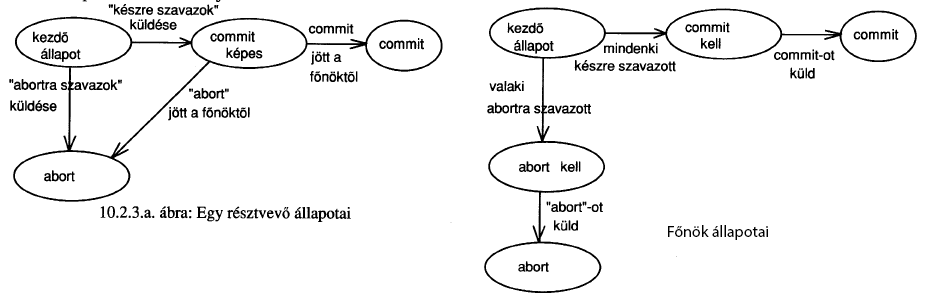
\includegraphics[scale=0.55]{img/2PC}

		\item \textbf{3 fázisú kész protokoll (3PC)} - "Blokkolásmentes"

			\forceindent Commit képes - Commit kész - COmmit

		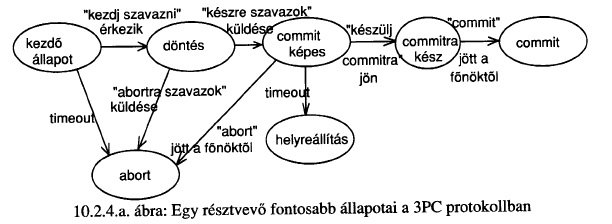
\includegraphics[scale=0.7]{img/3PC1}

		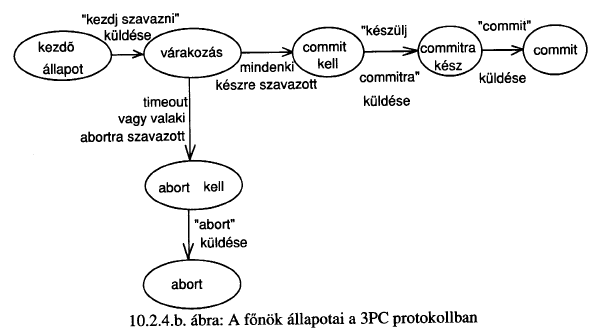
\includegraphics[scale=0.7]{img/3PC2}

		Értelmezés: Amikor egy résztvevő megkapja a "készülj commitra" üzenetet, akkor tudhatja, hogy mindenki készre szavazott. A résztvevők ezt nyugtázzák, ezután küldi a főnök a "commit jön" üzenetet. Ha egy résztvevő ezt is veszi, akkor ebből már tudja hogy minde résztvevő már megtudta, hogy minden résztvevő commitra szavazott. Ezután commitálhat.


	\end{enumerate}
